\documentclass[10pt, a4paper]{article}

\linespread{1} 
\usepackage{float}

\usepackage{geometry}
 \geometry{
 a4paper,
  total={122mm,193mm},
 left=44mm,
 right=44mm,
 bottom=52mm,
 top=52mm,
 }

\usepackage{amsfonts,amssymb,graphicx,color}
\usepackage{caption}
\usepackage{subcaption, multirow}

\usepackage{color, colortbl, framed}
\usepackage[T1]{fontenc}
\usepackage{mathptmx}

\usepackage{amsmath}
%\usepackage{lineno,hyperref}
\usepackage{authblk}
\usepackage{titlesec}

\usepackage{epstopdf}

\usepackage{hhline}
\usepackage{xcolor,colortbl}
\usepackage[sort&compress,square]{natbib}
\bibliographystyle{IJMRE_style}

% Do formatki
\usepackage{fancyhdr}
\newcommand{\helv}{%
\itshape \fontsize{9}{11}\selectfont}

 \lhead{\helv 27th International Symposium on Mine Planning and Equipment Selection, Santiago, Chile}

\captionsetup{justification   = raggedright,
              singlelinecheck = false}
              
\def\figurename{\bfseries Fig.}%
\def\tablename{\bfseries Table}%


\def\keywords#1{\par\addvspace\medskipamount{\rightskip=0pt plus1cm
\def\and{\ifhmode\unskip\nobreak\fi\ $\cdot$
}\noindent\keywordname\enspace\ignorespaces#1\par}}
 \def\keywordname{{\bfseries Keywords:}}%
%  \setcounter{secnumdepth}{0}
\usepackage{titlesec}
\titlespacing{\section}{0pt}{\parskip}{-\parskip}
\titlespacing{\subsection}{0pt}{\parskip}{-\parskip}
 \titleformat*{\section}{\normalfont\fontfamily{ptm}\fontsize{12}{19}\bfseries}
 \titleformat*{\subsection}{\normalfont\fontfamily{ptm}\fontsize{10}{18}\bfseries}
%  \setcounter{secnumdepth}{0}
\usepackage{titlesec}
\titlespacing{\section}{0pt}{\parskip}{-\parskip}
\titlespacing{\subsection}{0pt}{\parskip}{-\parskip}
 \titleformat*{\section}{\normalfont\fontfamily{ptm}\fontsize{10}{19}\bfseries}
 \titleformat*{\subsection}{\normalfont\fontfamily{ptm}\fontsize{10}{18}\bfseries}

\setlength{\columnsep}{6,3mm}
% \font\myfont=cmr12 at 24pt

\newcommand*{\myfont}{%
     \usefont{\encodingdefault}{\rmdefault}{n}{n}%
     \fontfamily{ptm}\fontsize{14}{20}\bfseries%
     \selectfont}
     
\newcommand*{\fontaut}{%
     \usefont{\encodingdefault}{\rmdefault}{n}{n}%
     \fontfamily{ptm}\fontsize{10}{10}%
     \selectfont}
     
\newcommand*{\fontaf}{%
     \usefont{\encodingdefault}{\rmdefault}{n}{n}%
     \fontfamily{ptm}\fontsize{9}{10}%
     \selectfont}


\renewcommand{\abstractname}{}    % clear the title

\title{\myfont \vspace{-5ex} Data acquisition system for position tracking and selected physiological and environmental parameters analysis to describe employee condition in underground mine}
% \author{}
\author[1]{\fontaut Pawe{\l} Stefaniak}
\author[1]{Jacek Wodecki}
\author[1]{Anna Michalak}
\author[1]{Agnieszka Wy{\l}oma{\'n}ska}
\author[1]{Rados{\l}aw Zimroz}

% \affil[1]{Faculty of Geoengineering, Mining and Geology, Wroclaw University of Science and Technology, Na Grobli 15, 50-421 Wroclaw, Poland\\ \{jacek.wodecki, radoslaw.zimroz\}@pwr.edu.pl}

\affil[1]{\fontaf KGHM Cuprum Ltd, Research and Development Centre, Sikorskiego 2-8, 53-659 Wroclaw, Poland\\ \{pkstefaniak, jwodecki, amichalak, awylomanska, rzimroz\}@cuprum.wroc.pl  \newline \textbf{Email of Corresponding author: awylomanska@cuprum.wroc.pl}  }

\date{} 

\begin{document}

\maketitle  \thispagestyle{fancy} 

\begin{abstract}
    \fontaf \vspace{-5ex}
\textbf{Abstract.} Nowadays some of raw materials are extracted from deposits in so called deep mines. Mining technology used for this process has not changed significantly, however environment becomes more and more harsh. It directly influences the comfort of people performing their tasks, especially in close distance to relatively poorly ventilated mining faces. Environmental conditions in the underground corridors might change relatively quickly. In addition, each person might be sensitive to given conditions at various level, it can also vary in time. In general, described problem might be associated with human fatigue and it has direct link to safety issues. Tackling such problem is a complex task. In this paper, we propose a portable monitoring system for an individual miner. It will measure and store locally the information about history of location of employee, his activity (walk, work, sitting, standing, etc.), his basic physiological parameters (temperature, pulse) as well as environmental parameters (temperature, humidity, gas presence). Black-box-type purpose of the system will allow to transfer recorded data to higher-level database after each shift. In this context it is essential to investigate long term trends rather than local disturbances. Most of data analysis is planned to be done in offline mode. However, for safety reason, some crucial parameters like $\mathrm{H_2S}$ or CO presence should be analyzed in real time to provide information about gas concentration in given mining cavity. The system should be lightweight, reliable and non-disturbing for miners. Authors propose to deploy the system using Arduino platform, which is cheap and commonly available technology. Moreover, miniaturization in sensor technology helps making the system as unnoticeable for the miner as possible.\\
 
\textbf{Keywords:} inertial measurement, monitoring system, activity detection, sensor fusion, underground mine
\end{abstract}

\section{Introduction}

Rapid development of communication and electronics systems enables to develop technology employed for tracking human physical activity and position together with change of physiological and environmental parameters. The harsh conditions of underground mine relate mainly to high temperature, humidity, dust, salinity and concentration of various gases in the air \cite{bascomptadetermination,hartman2012mine}. There exist many areas where levels of toxic gases (e.g. $\mathrm{H_2S}$ and CO) might locally exceed expected limit values. Furthermore, it needs to be pointed out that miners undergo intensified stress due to i.a. presence of many dangers to life or health in underground mine \cite{ryan2017heat}. Such working conditions in combination with medium or high energy expenditure may induce severe organism functioning disorders, in addition to increased body temperature and heart rate. As a further consequence, it may lead to limited physical fitness and motor coordination of workers \cite{dosinas2006measurement}.

This paper describes prototype development of the monitoring system to measure physical activity of miners, their health parameters as well as selected environmental parameters of their workplace including post-factum location in corridor. Similar solutions are well-known in the literature \cite{shaffer1992position,hol2007robust,sabatini2011estimating,aggarwal2011human,dosinas2006measurement,paiyarom2009activity,pantelopoulos2010survey}. Majority of them are dedicated to sport, healthcare sector but these application does not correspond to underground mine reality. Influence of miner physical activity on its physiological parameters in harsh and varying environmental conditions has not been recognized in detail yet. In the mining practice, applied methods of tracking miners are based on RFID technology what provides only data to identify their presence in certain zone without their position in three-dimensional space. In addition, application of inertial sensor allows to recognize type of performing physical activity.

It is also relevant to consider gas concentration analysis in mining air. Fusion of such data allows to perform context analysis which may deliver many information necessary to know unknown relationships between behaviours of an organism correspond to different physical activity forms in underground mine. On-going monitoring of air parameters allows to estimate real parameters of local atmosphere, regularities between these parameters and employee's tiredness or type of work.

In this paper we present a initial results of testing of measuring platform in underground mine in order to validate a technical functionality of measurement layer with the focus on the motion tracking, and to identify possible difficulties. The paper is organized as follows: after the introduction, concept and general requirements of the system are described in section \ref{s:req}, then design of the system is discussed in section \ref{s:design}, after that test of inertial measurements is described in section \ref{s:func}.

\section{Main requirements for the system}\label{s:req}

Requirements for the system assume technological simplicity, but are mostly driven by the need of measuring certain physical parameters of the environment and the workers themselves (see Fig. \ref{fig:idea}). 

\begin{figure}[ht!]
    \centering
    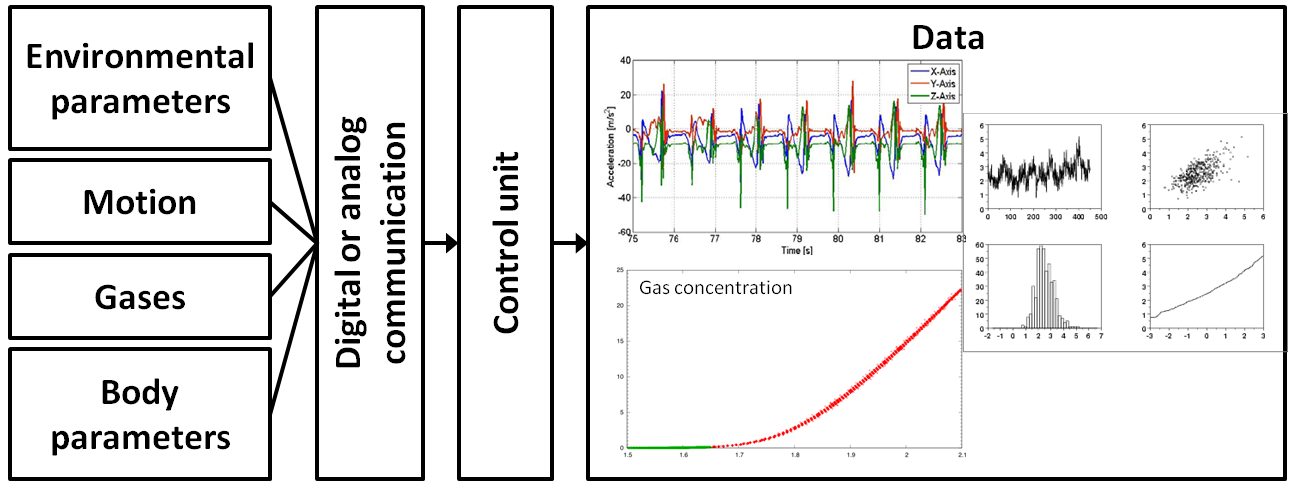
\includegraphics[width=\textwidth]{fig/idea.png}
    \caption{Functional concept of the system}
    \label{fig:idea}
\end{figure}

One of the main functionalities of the system is registering motion data that enable path reconstruction possible to be projected on a map. Example of such visualization is presented on Fig. \ref{fig:map}. In order to perform such measurements there is a need to employ so called Inertial Measurement Units (IMU), that consist of accelerometers, gyroscopes and magnetometers. Fusing raw data from those sensors using appropriate mathematical concepts allows to obtain displacement information which is necessary for path reconstruction.

\begin{table}[ht!]
    \centering
    \caption{Measured parameters}
  \begin{tabular}{|l|l|}
    \hline
    \textbf{Group} & \textbf{Parameter} \\ \hline
        \multirow{3}{8em}{Environmental parameters} & Air temperature \\ 
        & Air pressure \\
        & Air humidity \\ \hline
        \multirow{2}{8em}{Gases} & $\mathrm{H_2S}$ concentration \\
        & CO concentration \\ \hline
        \multirow{2}{8em}{Physiological parameters} & Body temperature \\ 
        & Pulse \\ \hline
        \multirow{2}{8em}{Motion parameters} & IMU on the head \\ 
        & IMU on the foot \\ \hline
    \end{tabular}
    \label{tab:tab1}
\end{table}

Beside recording motion data, it is also required to collect other types of information. Selected parameters are divided into four main groups (see Table \ref{tab:tab1}).

\section{System design}\label{s:design}

Taking into consideration requirements for the system, commercially available components have been selected to build the prototype (see Fig. \ref{fig:sensors} and Table \ref{tab:tab2}).

\begin{figure}[ht!]
    \centering
    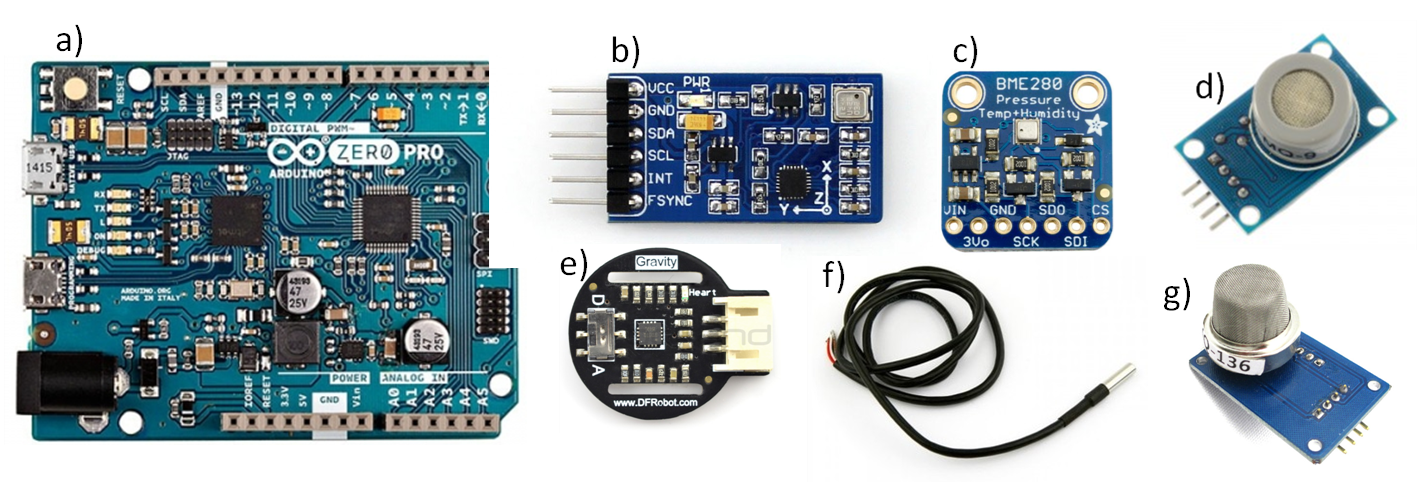
\includegraphics[width=\textwidth]{fig/sensors.png}
    \caption{Functional components of designed system, see Table \ref{tab:tab2}}
    \label{fig:sensors}
\end{figure}

\begin{table}[ht!]
    \centering
    \caption{System components}
  \begin{tabular}{|l|l|}
    \hline
    \textbf{Component} & \textbf{Role} \\ \hline
        a) Arduino M0 Pro & Control platform \\ \hline
        b) Waveshare IMU 10DoF & Inertial measurements \\ \hline
        \multirow{3}{9em}{c) Adafruit BME280} & Air temperature \\
        & Air pressure \\
        & Air humidity \\ \hline
        d) MQ-9 sensor & CO concentration \\ \hline
        e) DFRobot Gravity & Pulse \\ \hline
        f) DS18B20 sensor & Body temperature \\ \hline
        g) MQ136 sensor & $\mathrm{H_2S}$ concentration \\ \hline
    \end{tabular}
    \label{tab:tab2}
\end{table}

Elements have been assembled according to the architecture presented on Fig. \ref{fig:diagram}. Sensors measuring body parameters and gases' concentrations have been connected to Arduino board via analog bus, which simply reads voltage levels provided by the sensors. Remaining sensors communicate with the processor via digital buses: $\mathrm{I^2C}$ and SPI, that operate using their own standardized protocols.

Sample rates of individual parameters are also very important to consider. Since environmental and vital parameters are by definition slowly-varying processes, it is not necessary to perform such measurements with high speeds. Hence, for those values sample rate is set to 1 Hz. The only exception is the pulse. For the reasons of memory management pulse sensor operates in digital mode. It means that instead of transmitting complete data of the pulse wave (which requires appropriate processing afterwards to identify the pulse rate), sensor processes the data internally and only transmits a single data packet at each heartbeat. This method simplifies system integration and significantly reduces the amount of data to be transmitted and stored. Hence, pulse parameter has no constant sample rate, but is managed asynchronously with the mechanism known as "interrupts" that triggers the sample transmission as soon as the heartbeat is detected.

\begin{figure}[ht!]
    \centering
    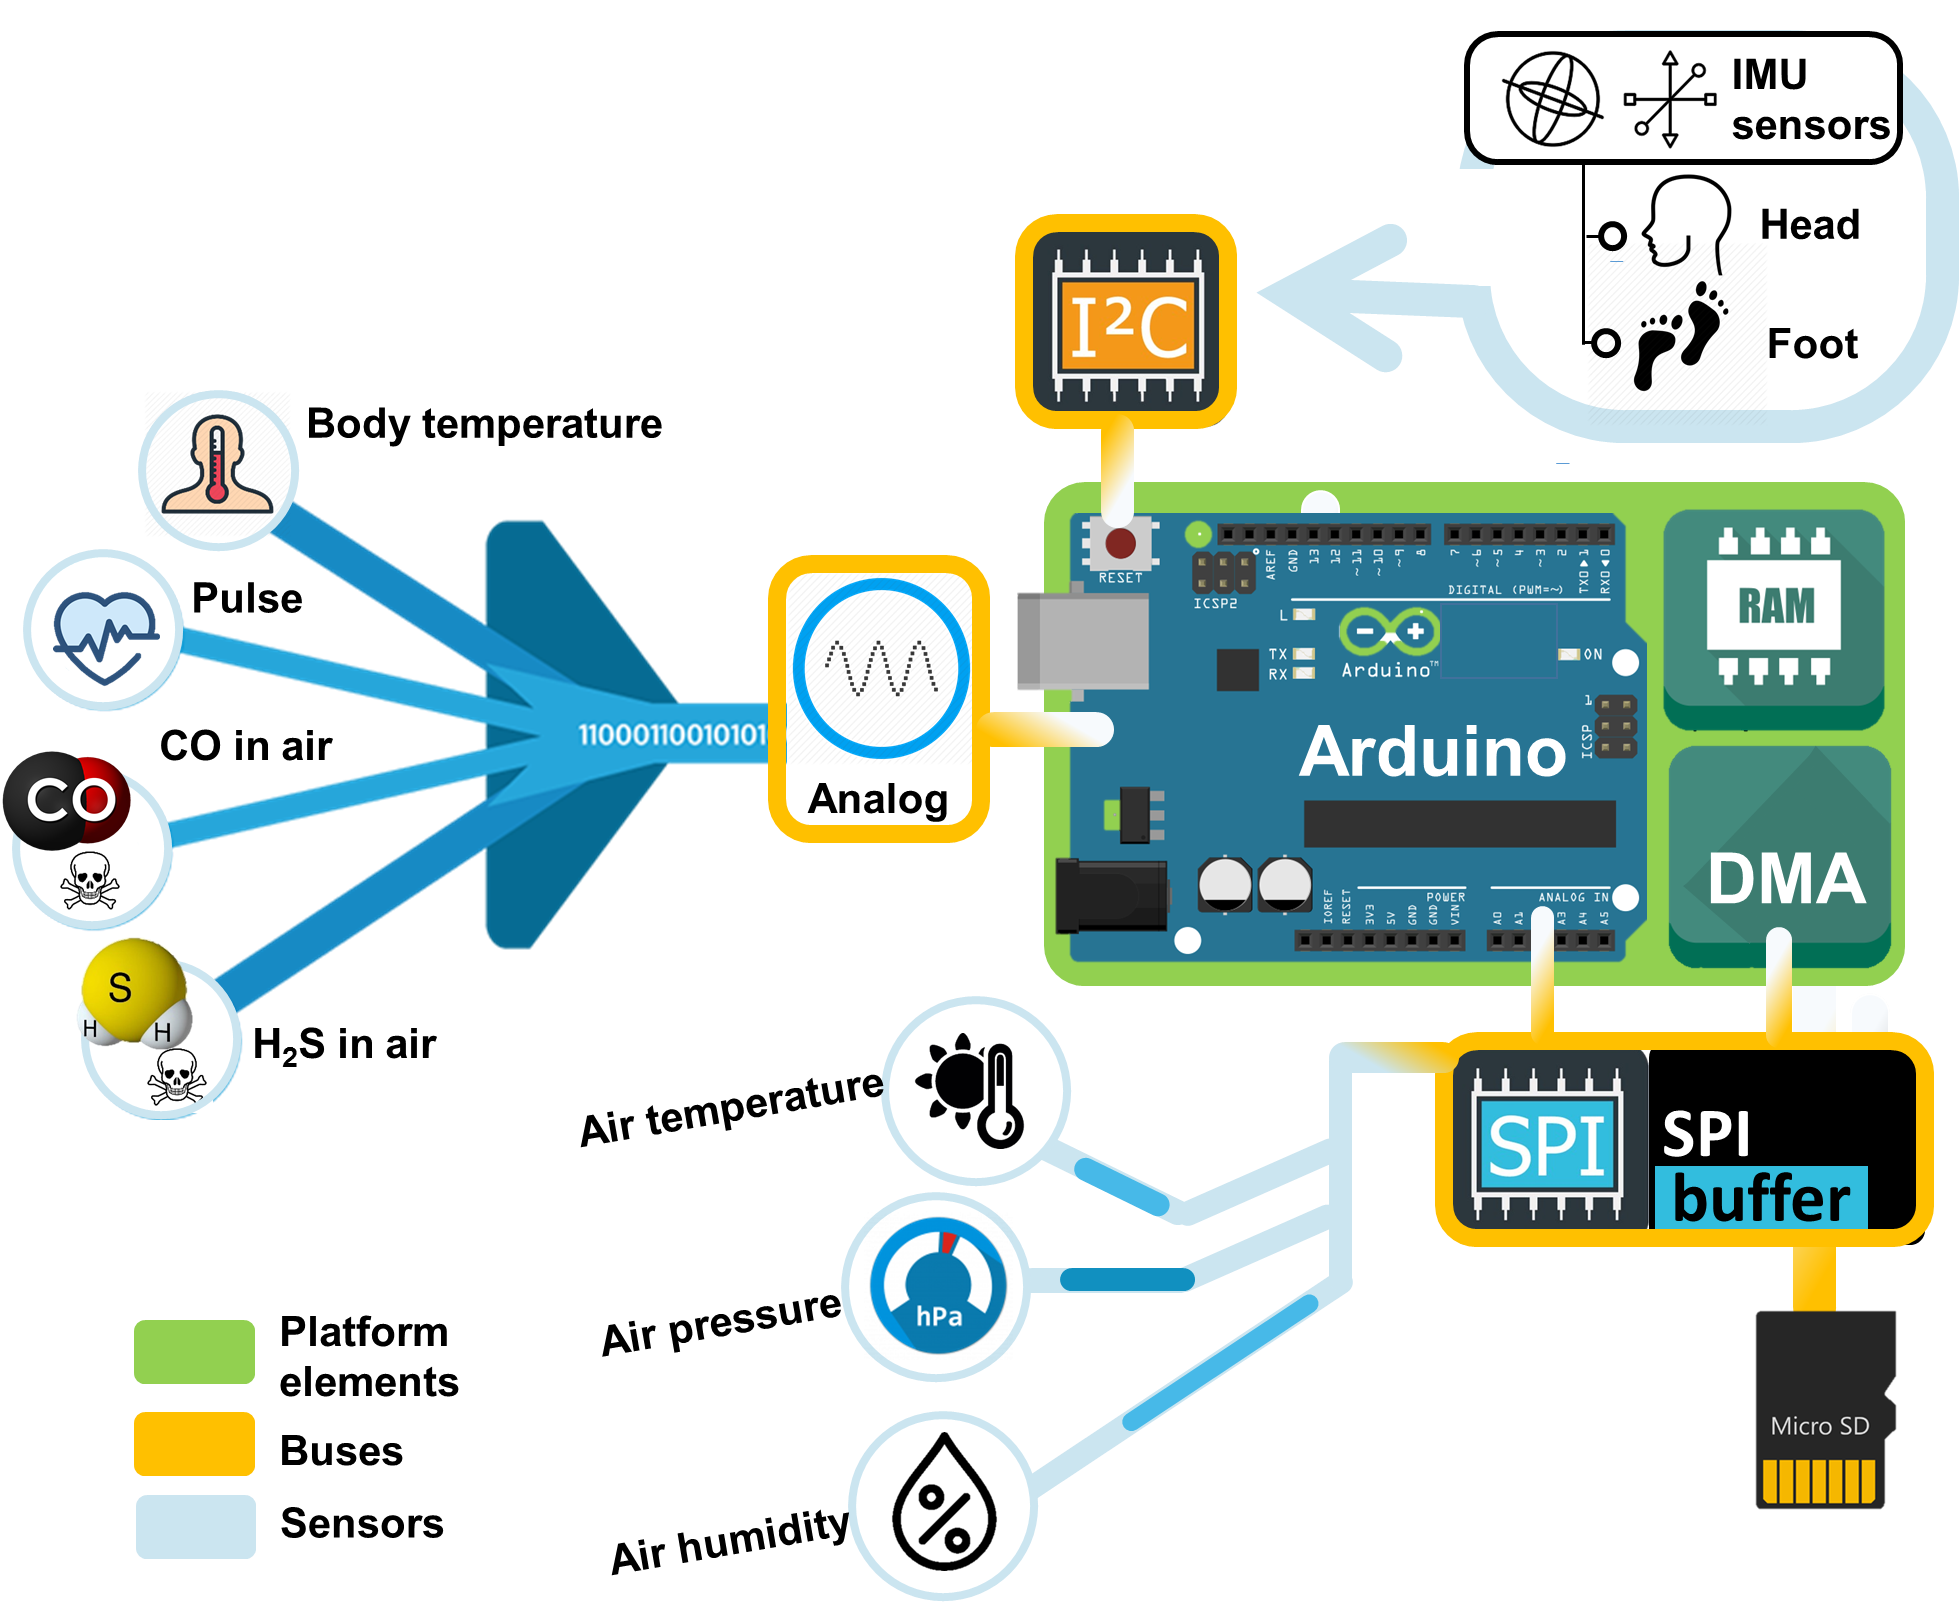
\includegraphics[width=.66\textwidth]{fig/fig3.png}
    \caption{System architecture}
    \label{fig:diagram}
\end{figure}

On the other hand, in case of motion measurements, it is crucial to capture every slightest movement of the sensor to be able to correctly reproduce motion trajectory. If any part of data is missing, motion trajectory will be completely incorrect. It is easiest to understand if one imagines that during the measurement, data acquisition fails when a person is making a turn while walking. In such case, data from before turning will be followed by data from after turning. Hence, from the data point of view, the turn never happened and person was walking straight ahead all the time. In such case everything that happened afterwards cannot be interpreted correctly and the entire measurement is invalid. Even a loss of data from very small movement will cause an avalanche effect on the following data, effectively corrupting it. Since such measurements are based on vibrations and rotations (which are varying very fast), it is crucial to sample the data with sufficiently high speeds. For practical reasons sample rate of IMU sensor was set to 100 Hz.

Another aspect of motion tracking is proper data interpretation. Since magnetic measurements are inapplicable in underground conditions, it is important to be able to operate on accelerometric and gyroscopic data only. However, values measured directly by sensors cannot be used for analysis, but have to "work together", hence there is a need to apply data fusion algorithm to appropriately convert raw data to so called \emph{linear accelerations} (interpretable equivalent of accelerometer data) and \emph{Euler angles} (interpretable equivalent of gyroscopic data). In such operation appropriate data smoothing is essential \cite{wodecki2018review}. This task is performed by employing Kalman-based AHRS (Altitude and Heading Reference System) algorithm \cite{marmion2006airborne}.

\section{Functionality testing of inertial measurements}\label{s:func}

\begin{figure}[ht!]
    \centering
    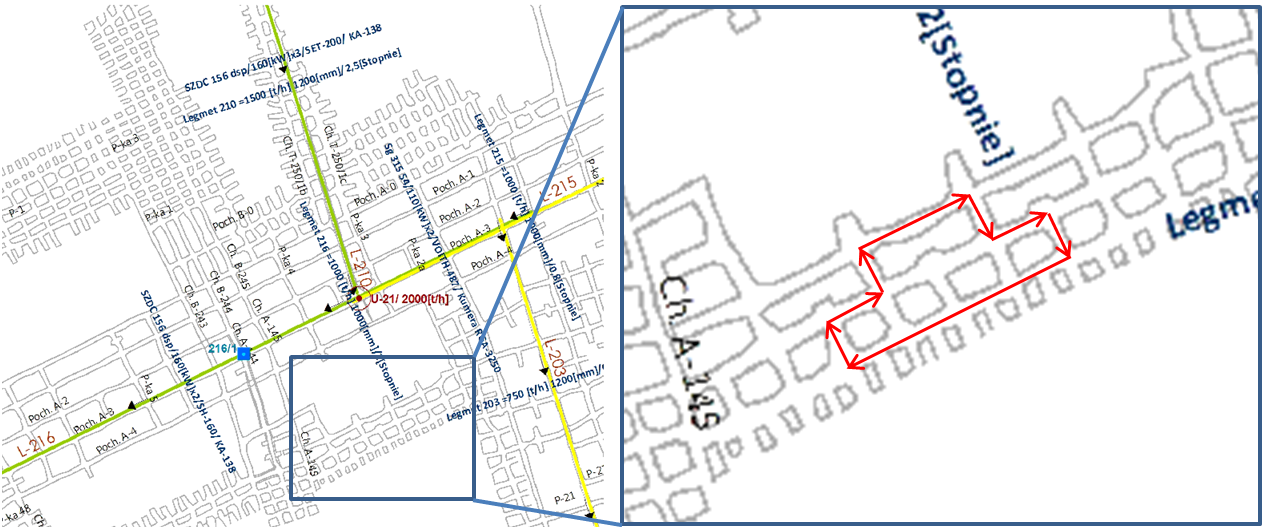
\includegraphics[width=\textwidth]{fig/map2.png}
    \caption{Example of desired data visualization}
    \label{fig:map}
\end{figure}

For practical reasons at this stage of development prototype testing was performed in a laboratory in easier, controlled environment. While slowly-varying processes (e.g. gases and other environmental and physiological parameters) impose no difficulties regarding registering and validation, in this paper authors focus on evaluation of the results of inertial measurements. In order to achieve that, detailed testing phase had to be conducted. It included calibrating the sensors themselves, establishing optimal filtering methods, stationary states elimination and many other signal-processing-related aspects of proper data acquisition and preprocessing. 

\begin{figure}[ht!]
    \centering
    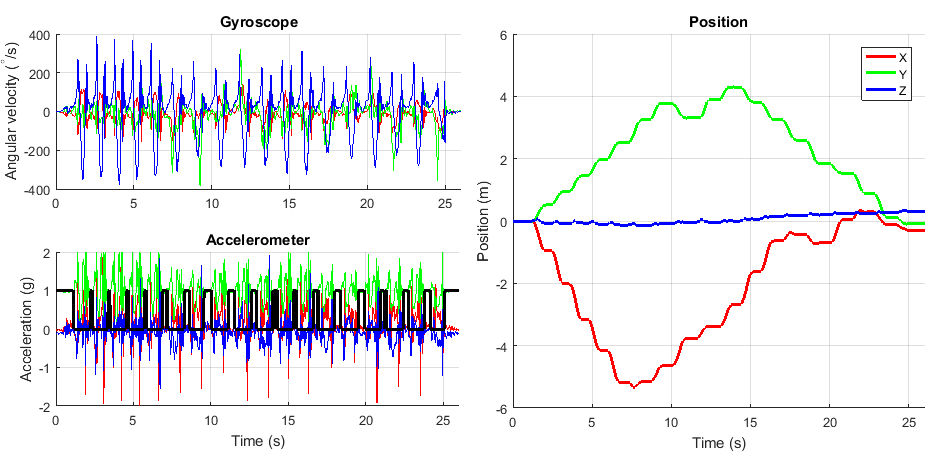
\includegraphics[width=.9\textwidth]{fig/IMUsignals.png}
    \caption{Exemplary inertial signals}
    \label{fig:sig}
\end{figure} 

After that, system had to be validated during a real measurement, and the aim of this phase is to determine if it is possible to obtain data that is possible to be correlated with the planned route. Authors selected test route based on the layout of underground corridors in the mine. Route has been mapped in the laboratory and person equipped with the acquisition system walked along it taking a measurement. Collected data has been superimposed on the planned route (see Fig. \ref{fig:map3}). Green arrows in Fig. \ref{fig:map3} corresponds to red ones in Fig. \ref{fig:map}. 

\begin{figure}[ht!]
    \centering
    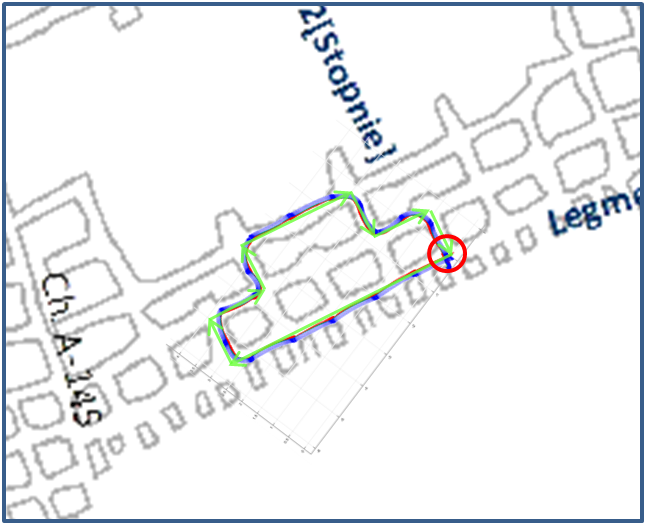
\includegraphics[width=.7\textwidth]{fig/map3.png}
    \caption{Route correlation experiment. Green arrows denote segments of planned route, blue data is a set of versors for the measured points and red circle is the point of start and finish.}
    \label{fig:map3}
\end{figure}

As a result, one can see that registered route corresponds almost perfectly to the planned one. Some level of roundness in registered route comes from the internal drift of a gyroscope. It is already reduced by a large amount by calibrating the sensor as well as possible and introducing selective drift elimination in the postprocessing algorithm, but in reality it is practically impossible to eliminate it completely.



\section{Conclusions}
Safety is one of the most regarded aspects of mine operation in recent decades. One of the investigated direction in this area is the analysis of working conditions for the miners. It involves environment assessment, as well as investigating workers vital parameters and location in the mine. Since wireless telecommunication in underground corridors is almost impossible to maintain for technological reasons (even wired communication is limited to an emergency landlines), it is impractical for now to deploy online monitoring system that transmits data from the sensors in real time. To address this difficulty, offline monitoring system has been proposed. It registers basic environmental parameters, miners vital functions and their relative position in three-dimensional space. System has been tested in laboratory conditions with satisfying results. Further work includes performing tests in real-life mining conditions underground, as well as further software-wise system optimization.

\bibliography{mybibfile}
\end{document}